\graphicspath{ {images/csv_dumps/} }
\section{CSV"=выгрузки} \label{sec:csv_dumps}

Раздел <<Мои выгрузки>> доступен из меню <<Мой профиль>> пользователю, у которого имеется хотя бы одна роль в рамках какого-либо университета. Конкретная выгрузка в списке доступна её автору только если у пользователя есть любое право в рамках привязанного к выгрузке университета.

\begin{figure}[H]
	\center{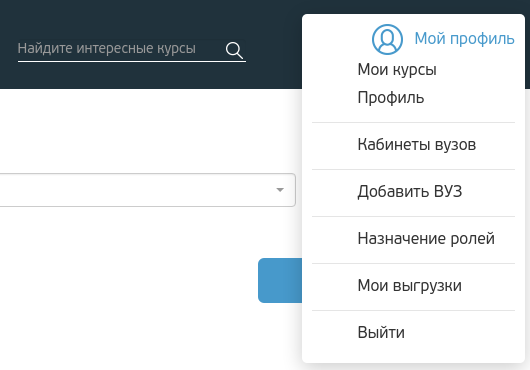
\includegraphics[width=1\linewidth]{my_dumps}}
	\caption{Переход в раздел <<Мои выгрузки>>}
	\label{img:employee:my_dumps}
\end{figure}

В целом данный раздел также представляет собой табличные данные с возможностью фильтрации, поиска, сортировки и выгрузки.
Более подробно эти возможности описаны в подразделе~\ref{sec:datatables}. Таблица с CSV"=выгрузками для готовых выгрузок 
содержит следующие специальные колонки:
\begin{itemize}
	\item \vcenteredinclude[height=25px]{save_csv} "--- скачать ранее сформированную выгрузку;
	\item \vcenteredinclude[height=25px]{more_csv} "--- подробности о выгрузке (применённые фильтры, сортировки и пр.,
	см.\ рис.~\ref{img:csv_dumps:details_csv});
	\item \vcenteredinclude[height=25px]{remove_csv} "--- удалить ранее сформированную выгрузку (появляется диалог подтверждения,
	см.\ рис.~\ref{img:csv_dumps:confirm_remove_csv});
\end{itemize}

\begin{figure}[H]
	\center{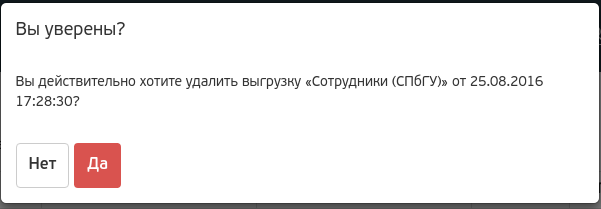
\includegraphics[width=1\linewidth]{confirm_remove_csv}}
	\caption{Диалог подтверждения удаления}
	\label{img:csv_dumps:confirm_remove_csv}
\end{figure}
\begin{figure}[H]
	\center{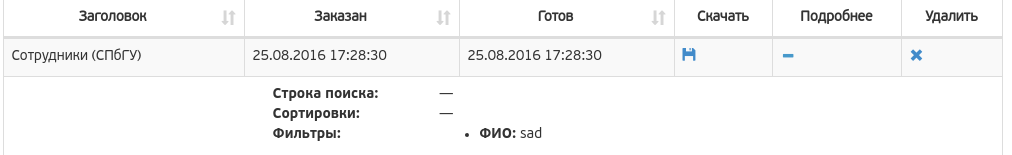
\includegraphics[width=1\linewidth]{details_csv}}
	\caption{Подробности о выгрузке}
	\label{img:csv_dumps:details_csv}
\end{figure}
